\documentclass[12pt]{article}
\textheight 23.5cm \textwidth 15.8cm
\topmargin -1.5cm \oddsidemargin 0.3cm \evensidemargin -0.3cm
\usepackage{tikz,mathpazo}
\usepackage{amsmath}
\usepackage{amssymb}
\usepackage{graphicx}
\usepackage[UTF8]{ctex}
\usepackage{amsmath}
\usepackage{amsthm}
\usepackage{amssymb}
\usepackage{mathrsfs}
\usepackage{multirow}
\usepackage{verbatim}
\usepackage{subfigure}
\usepackage{color}
\usepackage{enumerate}
\usepackage{geometry}


\usepackage[colorlinks,            
linkcolor=red,            
anchorcolor=blue,            
citecolor=green            
]{hyperref} %超链接
%  超链接用法示范例:For further references see \href{http://www.overleaf.com}{Something Linky} or go to the next url: \url{http://www.overleaf.com}


\begin{document}

\begin{center}
\huge\textbf{ASAP/ARAP 网格参数化}
\end{center}



\section{数学原理}
在第四次实验中我们实现了把网格边界固定到平面图多边形上的参数化,本次实验中要做的ASAP/ARAP参数化是不固定边界的参数化。

我们先把曲面三角网格的每一个三角形独立地保形地铺到平面上,再把这些三角形拼成一个平面三角形网格。
\begin{figure}[htb]
\centering
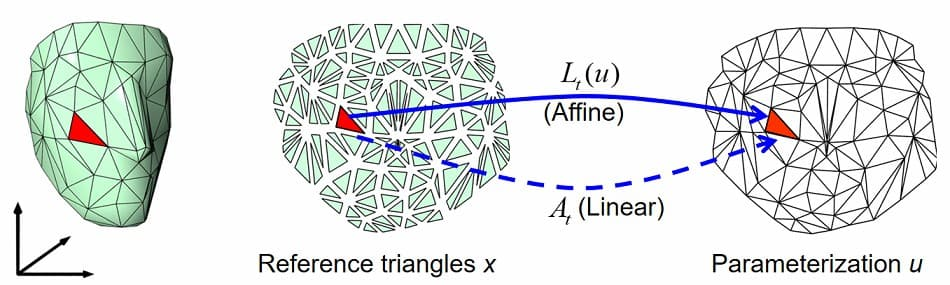
\includegraphics[height=1.5in]{1.jpg}
\end{figure}

拼成平面网格的过程势必会造成三角形扭曲,这个过程其实是对每个三角形$x_t=\{x_t^0,x_t^1,x_t^2\}$做仿射变换得到三角形$u_t=\{u_t^0,u_t^1,u_t^2\}$,设这个仿射变换的线性部分为$J_t(u)$。我们希望$J_t(u)$和一类我们允许的线性变换M(比如旋转、放缩)最接近,因此我们定义能量:
\begin{align*}E(u,L)=&\sum\limits_{t=1}^T\Delta_t||J_t(u)-L_t||_F^2\\
 =&\frac12\sum\limits_{t=1}^T\sum\limits_{i=0}^2 cot(\theta_t^{i+2})||(u_t^i-u_t^{i+1})-L_t(x_t^i-x_t^{i+1})||^2  \end{align*}

其中,$L=\{L_1,L_2,...,L_T\},L_t\in M;
\Delta_t $是三角形$ x_t$ 的面积$;\theta_t^i$是三角形$x_t$中顶点$x_t^{i}$所在的角。ASAP/ARAP接下来要做的就是求$u_t,L_t(u)$使得这个能量最小。


\subsection{ASAP}
$M=\left\{  \begin{pmatrix}a & b\\-b & a\end{pmatrix}:a,b\in \mathbf{R}\right\}$

$E(u,L)$对$a,b,u$求导得:
$$\frac{\partial E}{\partial a_t}=\sum\limits_{i=0}^2 cot(\theta_t^{i+2})(a_t[(\Delta x_{t,x}^i)^2+(\Delta x_{t,y}^i)^2]-\Delta x_{t,x}^i\Delta u_{t,x}^i-\Delta x_{t,y}^i\Delta u_{t,y}^i)$$
$$\frac{\partial E}{\partial b_t}=\sum\limits_{i=0}^2 cot(\theta_t^{i+2})(b_t[(\Delta x_{t,x}^i)^2+(\Delta x_{t,y}^i)^2]-\Delta x_{t,y}^i\Delta u_{t,x}^i+\Delta x_{t,x}^i\Delta u_{t,y}^i)$$

$$\frac{\partial E}{\partial u_x^{[k]}}=\sum\limits_{(i,t)\in N(u^{[k]})} cot(\theta_t^{i-1})(-a_t\Delta x_{t,x}^i-b_t\Delta x_{t,y}^i+\Delta u_{t,x}^i)- cot(\theta_t^{i+1})(-a_t\Delta x_{t,x}^{i-1}-b_t\Delta x_{t,y}^{i-1}+\Delta u_{t,x}^{i-1})$$
$$\frac{\partial E}{\partial u_y^{[k]}}=\sum\limits_{(i,t)\in N(u^{[k]})} cot(\theta_t^{i-1})(-a_t\Delta x_{t,y}^i+b_t\Delta x_{t,x}^i+\Delta u_{t,y}^i)- cot(\theta_t^{i+1})(-a_t\Delta x_{t,y}^{i-1}+b_t\Delta x_{t,x}^{i-1}+\Delta u_{t,y}^{i-1})$$


其中,下标t代表第t个三角形,上标i代表三角形中的第i个点,下标x,y代表点坐标的x,y分量,$\Delta x_t^i=x_t^i-x_t^{i+1},N(u^{[k]})=\{(i,t):u^{[k]}=u_t^i\}$.

令所有导数都为0,解方程。

构造方程时要固定两个点,否则会得到平凡解,我固定了边界的第一个点和中位点分别到(0,0),(1,1).

实际构造方程组时,对$\sum\limits_{(i,t)\in N(u^{[k]})}$无需遍历顶点找相邻三角形,可以与$\frac{\partial E}{\partial a_t},\frac{\partial E}{\partial b_t}$一样遍历三角形。


\subsection{ARAP}
$M=\left\{  \begin{pmatrix}cos\theta & sin\theta\\-sin\theta & cos\theta \end{pmatrix}:\theta\in  [0,2\pi)  \right\}$

对此问题,我们使用Local/Global方法。

1、首先用ASAP方法初始化u,

2、Local阶段:固定u,求L使E最小。在这里,我们也可以用$S_t(u)=\\\sum\limits_{i=0}^2cot(\theta_t^i)(\Delta u_t^i)(\Delta x_t^i)^T$ 来代替$J_t(u)$. 做奇异值分解$S_t(u)=U\Sigma V^T$ (此处奇异值分解是一个"signed version",即允许$\sigma_2$为负,但要保证$UV^T$的行列式为正),再令$L_t:=UV^T.$\

3、Global 阶段:固定L,求u使E最小。

解方程组:
$$\sum\limits_{j\in N(i)}[cot(\theta_{ij})+cot(\theta_{ji})](u_i-u_j)=\sum\limits_{j\in N(i)}[cot(\theta_{ij})L_{t(i,j)}+cot(\theta_{ji})L_{t(j,i)}](x_i-x_j)$$

其中,$\theta_{ij}$是半边(i,j)所在三角形中半边(i,j)所对的角,$t(i,j)$是半边(i,j)所在的三角形。

构造方程时固定边界的第一个点到(0,0)。

4、多次重复Local,Global阶段。每次迭代,能量E(u,L)都不增,因此会收敛到能量极小的情况。


\section{结果展示}
\begin{table*}[htb]
\begin{center}
\begin{tabular}{|c|c|c|}
  \hline
  原网格 &ASAP &ARAP(迭代10次) \\\hline

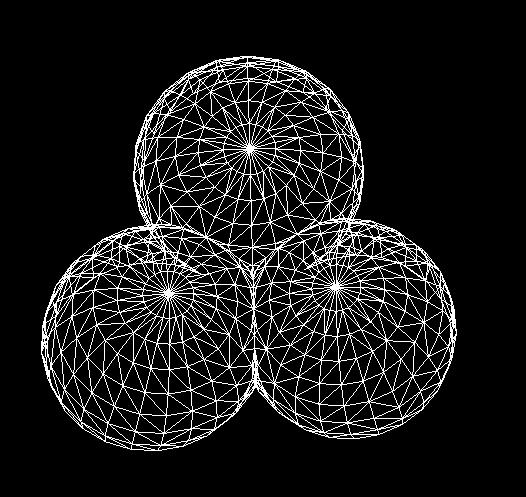
\includegraphics[height=1.5in]{10.png}&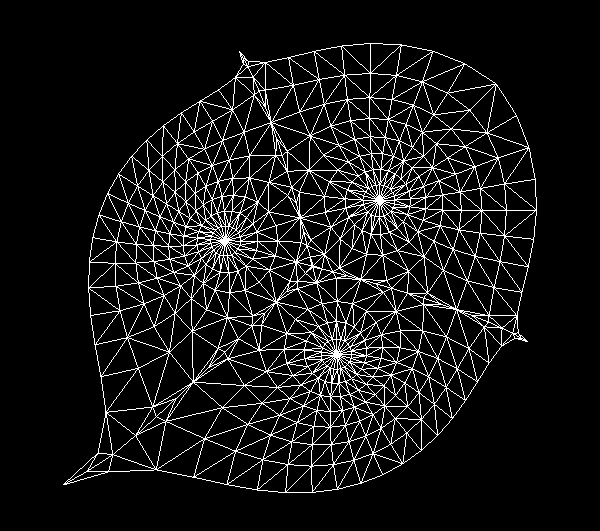
\includegraphics[height=1.5in]{11.png}&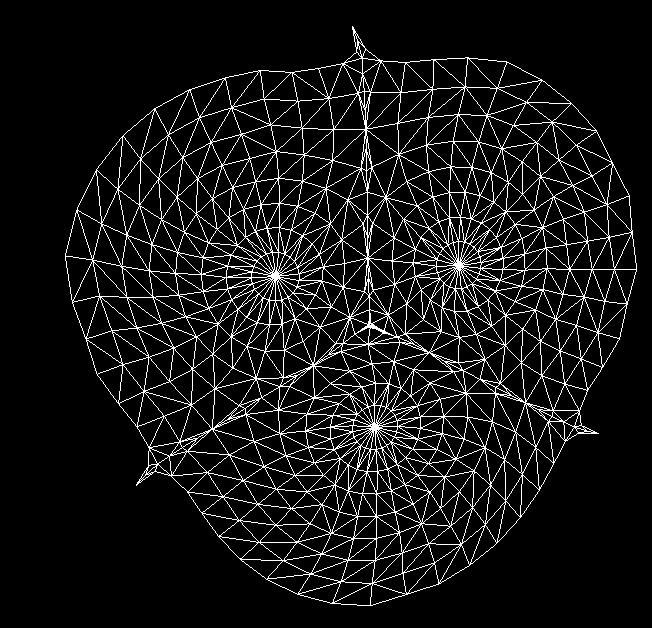
\includegraphics[height=1.5in]{12.png}\\
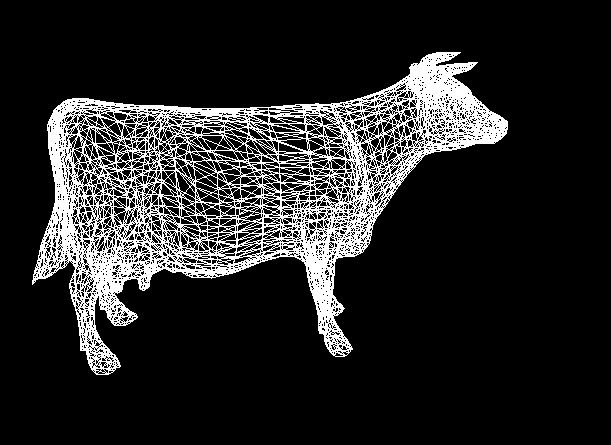
\includegraphics[height=1.5in]{20.png}&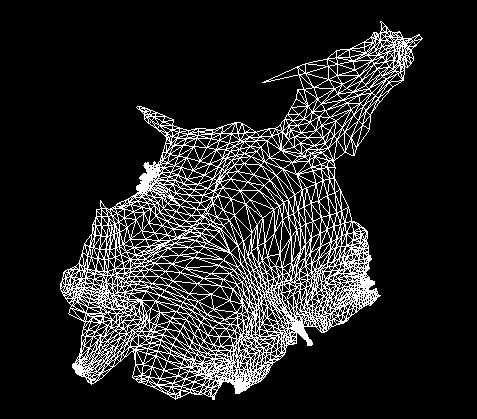
\includegraphics[height=1.5in]{21.png}&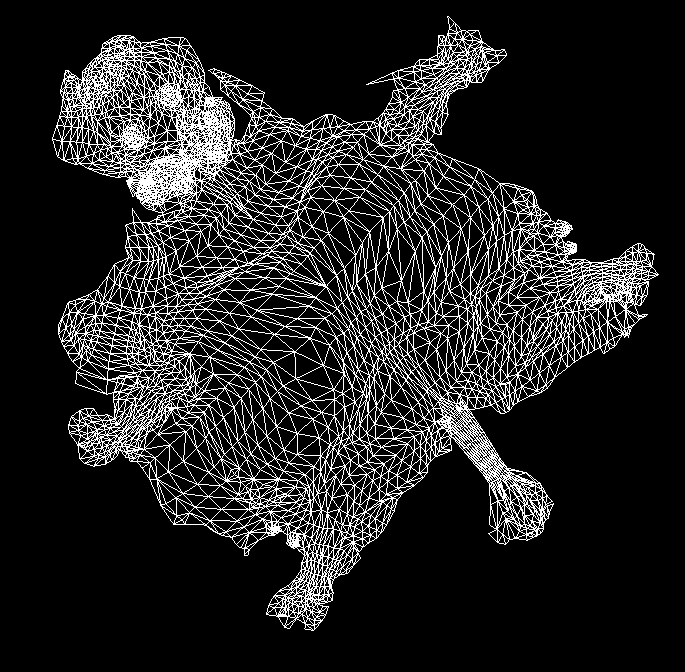
\includegraphics[height=1.5in]{22.png}\\\hline

\end{tabular}
\end{center}
\end{table*}



\begin{table*}[htb]
\begin{center}
\begin{tabular}{|c|c|c|c|}
  \hline
  固定边界(uniform) &固定边界(cot)&ASAP &ARAP(迭代10次) \\\hline

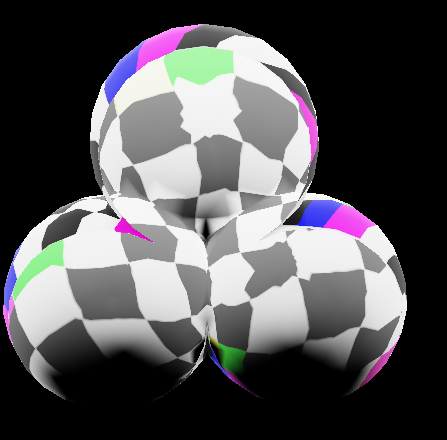
\includegraphics[height=1in]{13.png}&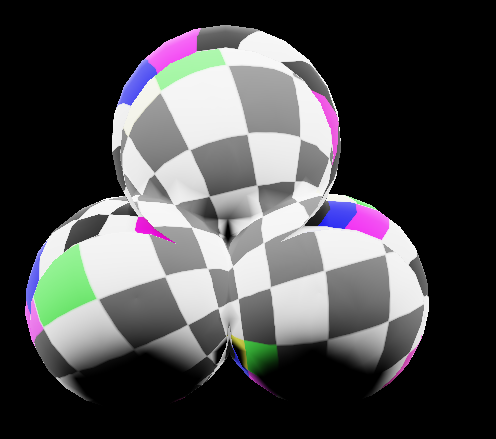
\includegraphics[height=1in]{14.png}&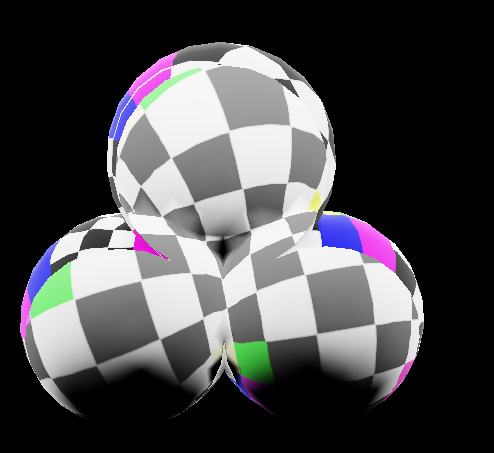
\includegraphics[height=1in]{15.png}&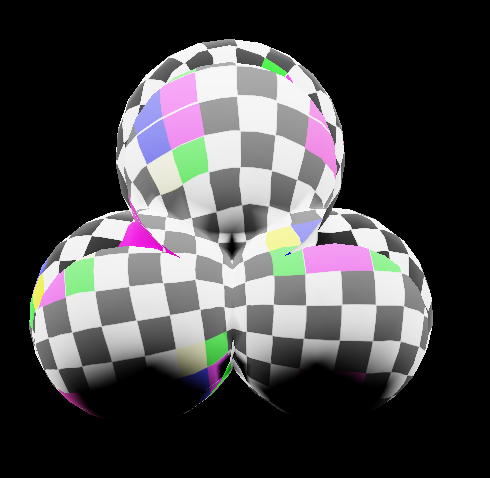
\includegraphics[height=1in]{16.png}\\
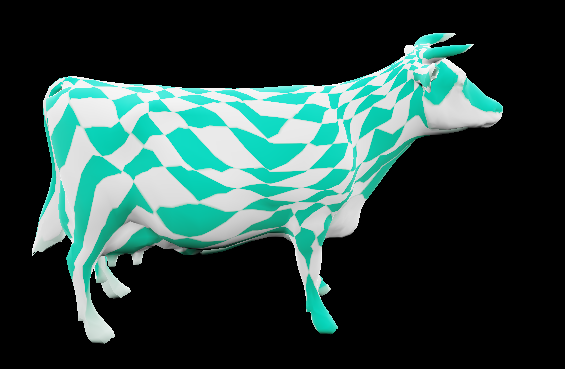
\includegraphics[height=1in]{23.png}&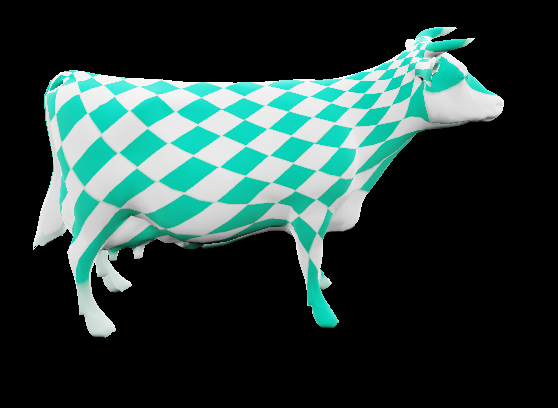
\includegraphics[height=1in]{24.png}&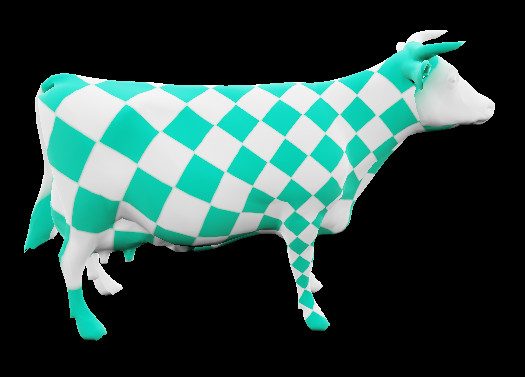
\includegraphics[height=1in]{25.png}&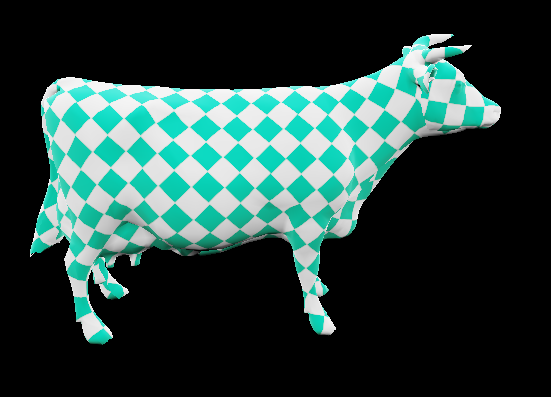
\includegraphics[height=1in]{26.png}\\
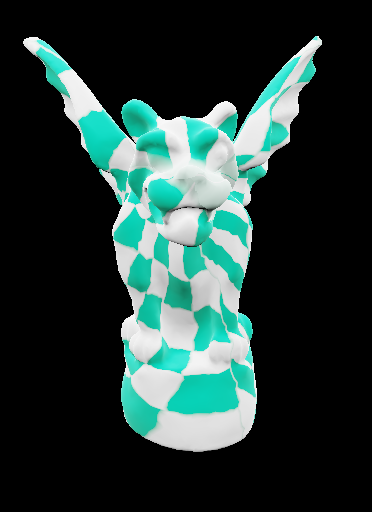
\includegraphics[height=1in]{33.png}&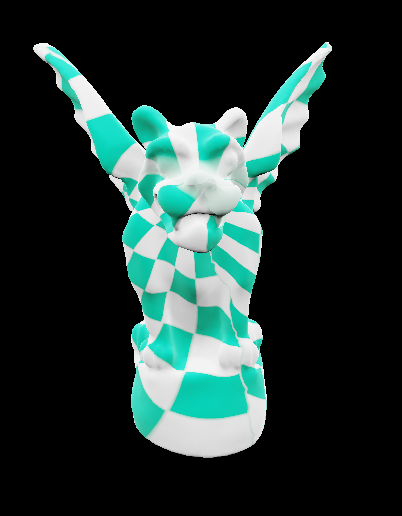
\includegraphics[height=1in]{34.png}&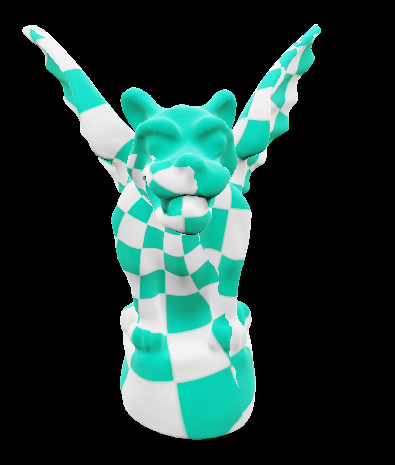
\includegraphics[height=1in]{35.png}&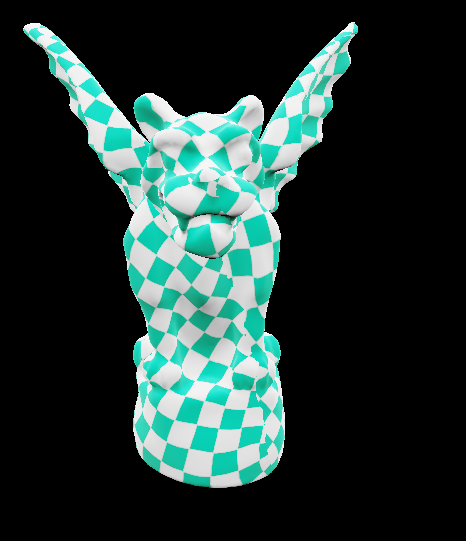
\includegraphics[height=1in]{36.png}\\
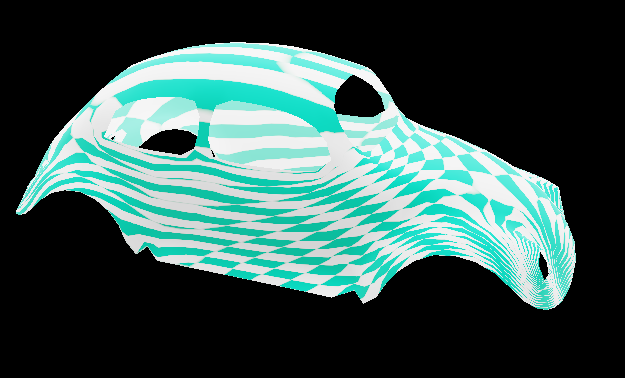
\includegraphics[height=1in]{43.png}&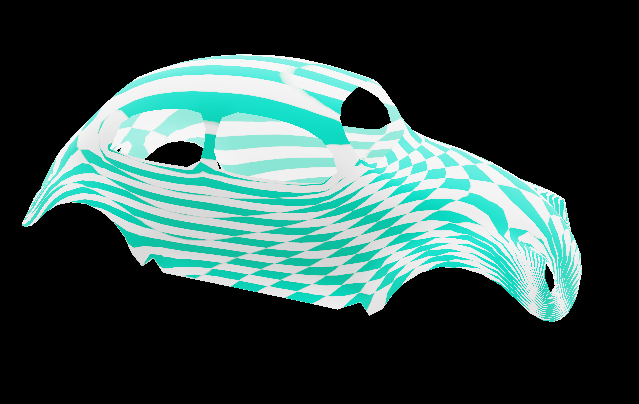
\includegraphics[height=1in]{44.png}&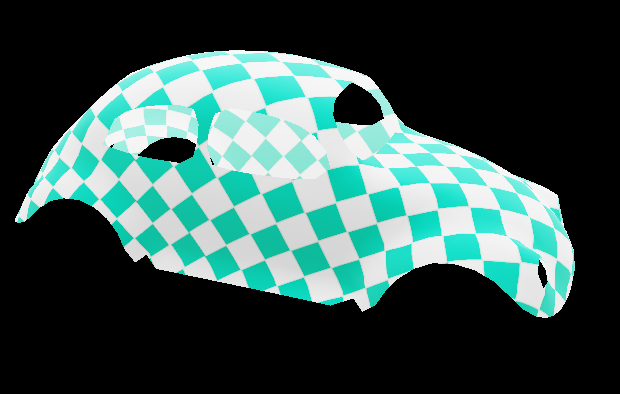
\includegraphics[height=1in]{45.png}&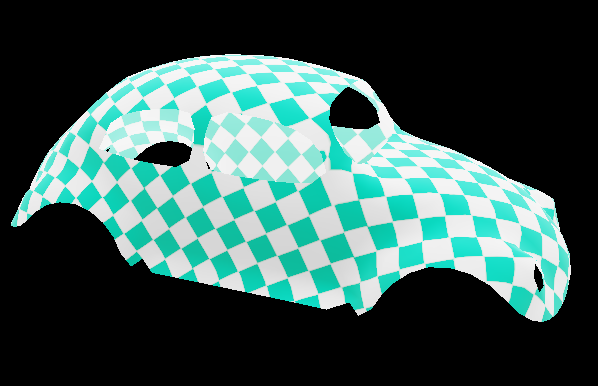
\includegraphics[height=1in]{46.png}\\\hline

\end{tabular}
\end{center}
\end{table*}

\end{document}